% !TEX program = pdflatex
% SIMC 2026 sample-problem report: Who are colluding?
% Tasks 1-5 with a focus on quantitative diagnostics and an
% innovative cluster-selection criterion.

\documentclass[11pt,a4paper]{article}

% ------------------------------------------------------------------
%  Packages
% ------------------------------------------------------------------
\usepackage[margin=1in]{geometry}
\usepackage{amsmath,amssymb,amsthm}
\usepackage{mathtools}
\usepackage{bm}
\usepackage{graphicx}
\usepackage{booktabs}
\usepackage{caption}
\usepackage{subcaption}
\usepackage{xcolor}
\usepackage[most]{tcolorbox}
\usepackage{siunitx}
\usepackage{enumitem}
\usepackage{hyperref}
\hypersetup{colorlinks=true, linkcolor=blue!50!black,
            citecolor=blue!50!black, urlcolor=blue!50!black}

% ------------------------------------------------------------------
%  Style: coloured "insight" and "result" boxes
% ------------------------------------------------------------------
\newtcolorbox{insight}[1][]{enhanced, breakable,
  colback=blue!4, colframe=blue!55!black, boxrule=0.6pt,
  arc=2pt, left=8pt, right=8pt, top=6pt, bottom=6pt,
  fonttitle=\bfseries, title=#1}

\newtcolorbox{keyresult}[1][]{enhanced, breakable,
  colback=red!4, colframe=red!55!black, boxrule=0.6pt,
  arc=2pt, left=8pt, right=8pt, top=6pt, bottom=6pt,
  fonttitle=\bfseries, title=#1}

% ------------------------------------------------------------------
%  Macros
% ------------------------------------------------------------------
\newcommand{\X}{\bm{X}}
\newcommand{\Sm}{\bm{S}}
\newcommand{\Exp}{\mathbb{E}}
\newcommand{\Var}{\mathrm{Var}}
\renewcommand{\Pr}{\mathbb{P}}
\DeclareMathOperator{\sign}{sign}

% ------------------------------------------------------------------
%  Title
% ------------------------------------------------------------------
\title{\bfseries Who Are Colluding? \\
       \large A Linear-Algebraic and Statistical Audit of Test-Taking Behaviour \\
       \normalsize SIMC 2026 Sample Problem -- Tasks 1 through 5}
\author{}
\date{\today}

\begin{document}
\maketitle

\begin{abstract}
We treat the question \emph{``which students colluded during a test?''} as a
geometry problem on the design matrix $\X\in\{-1,+1\}^{M\times N}$. Tasks~1
and~2 visualise $\X$ and the Gram matrix $\Sm = \X\X^{\!\top}$, immediately
exposing one pair of students (indices $5$ and $10$) whose answer vectors
are \emph{identical}. Task~3 applies $K$-means to recover the underlying
group structure, and we introduce a \textbf{singleton-filtered silhouette
criterion} that resolves the well-known tendency of the silhouette score
to reward over-fragmentation. Task~4 makes the qualitative case for
collusion. Task~5 closes the section by deriving the closed-form mean
$\langle S\rangle = N(2p-1)^2$ and standard deviation
$\sigma_N = \sqrt{N\bigl[1 - (2p-1)^4\bigr]}$ of the similarity score under
a null hypothesis of independent test-takers; these will anchor the
hypothesis tests of Tasks~6--8.
\end{abstract}

\tableofcontents
\vspace{1em}\hrule\vspace{1em}

% ==================================================================
\section{Task 1 -- The Design Matrix}
% ==================================================================

\subsection{Definition and encoding}
Let there be $M$ students and $N$ questions. The \emph{design matrix} is
\begin{equation}
  \X \;\equiv\; X_{ij} \;\in\; \{-1,+1\}^{M\times N},
  \qquad
  X_{ij} \;=\;
  \begin{cases}
    +1, & \text{student $i$ answered question $j$ correctly,}\\
    -1, & \text{otherwise.}
  \end{cases}
  \label{eq:design}
\end{equation}
The symmetric $\pm 1$ encoding (rather than $\{0,1\}$) is deliberate: it
makes Eq.~\eqref{eq:design} a sign-vector representation, so that the
inner product of two rows directly measures \emph{net agreement} (see
Task~2).

\subsection{Visualisation}
Figure~\ref{fig:task1} shows the small subset
\texttt{sample\_small}$\in\{-1,+1\}^{50\times 25}$ rendered as a binary
heatmap, with marginal bar plots of the per-student total
$\sum_j X_{ij}$ and per-question total $\sum_i X_{ij}$.

\begin{figure}[htb]
  \centering
  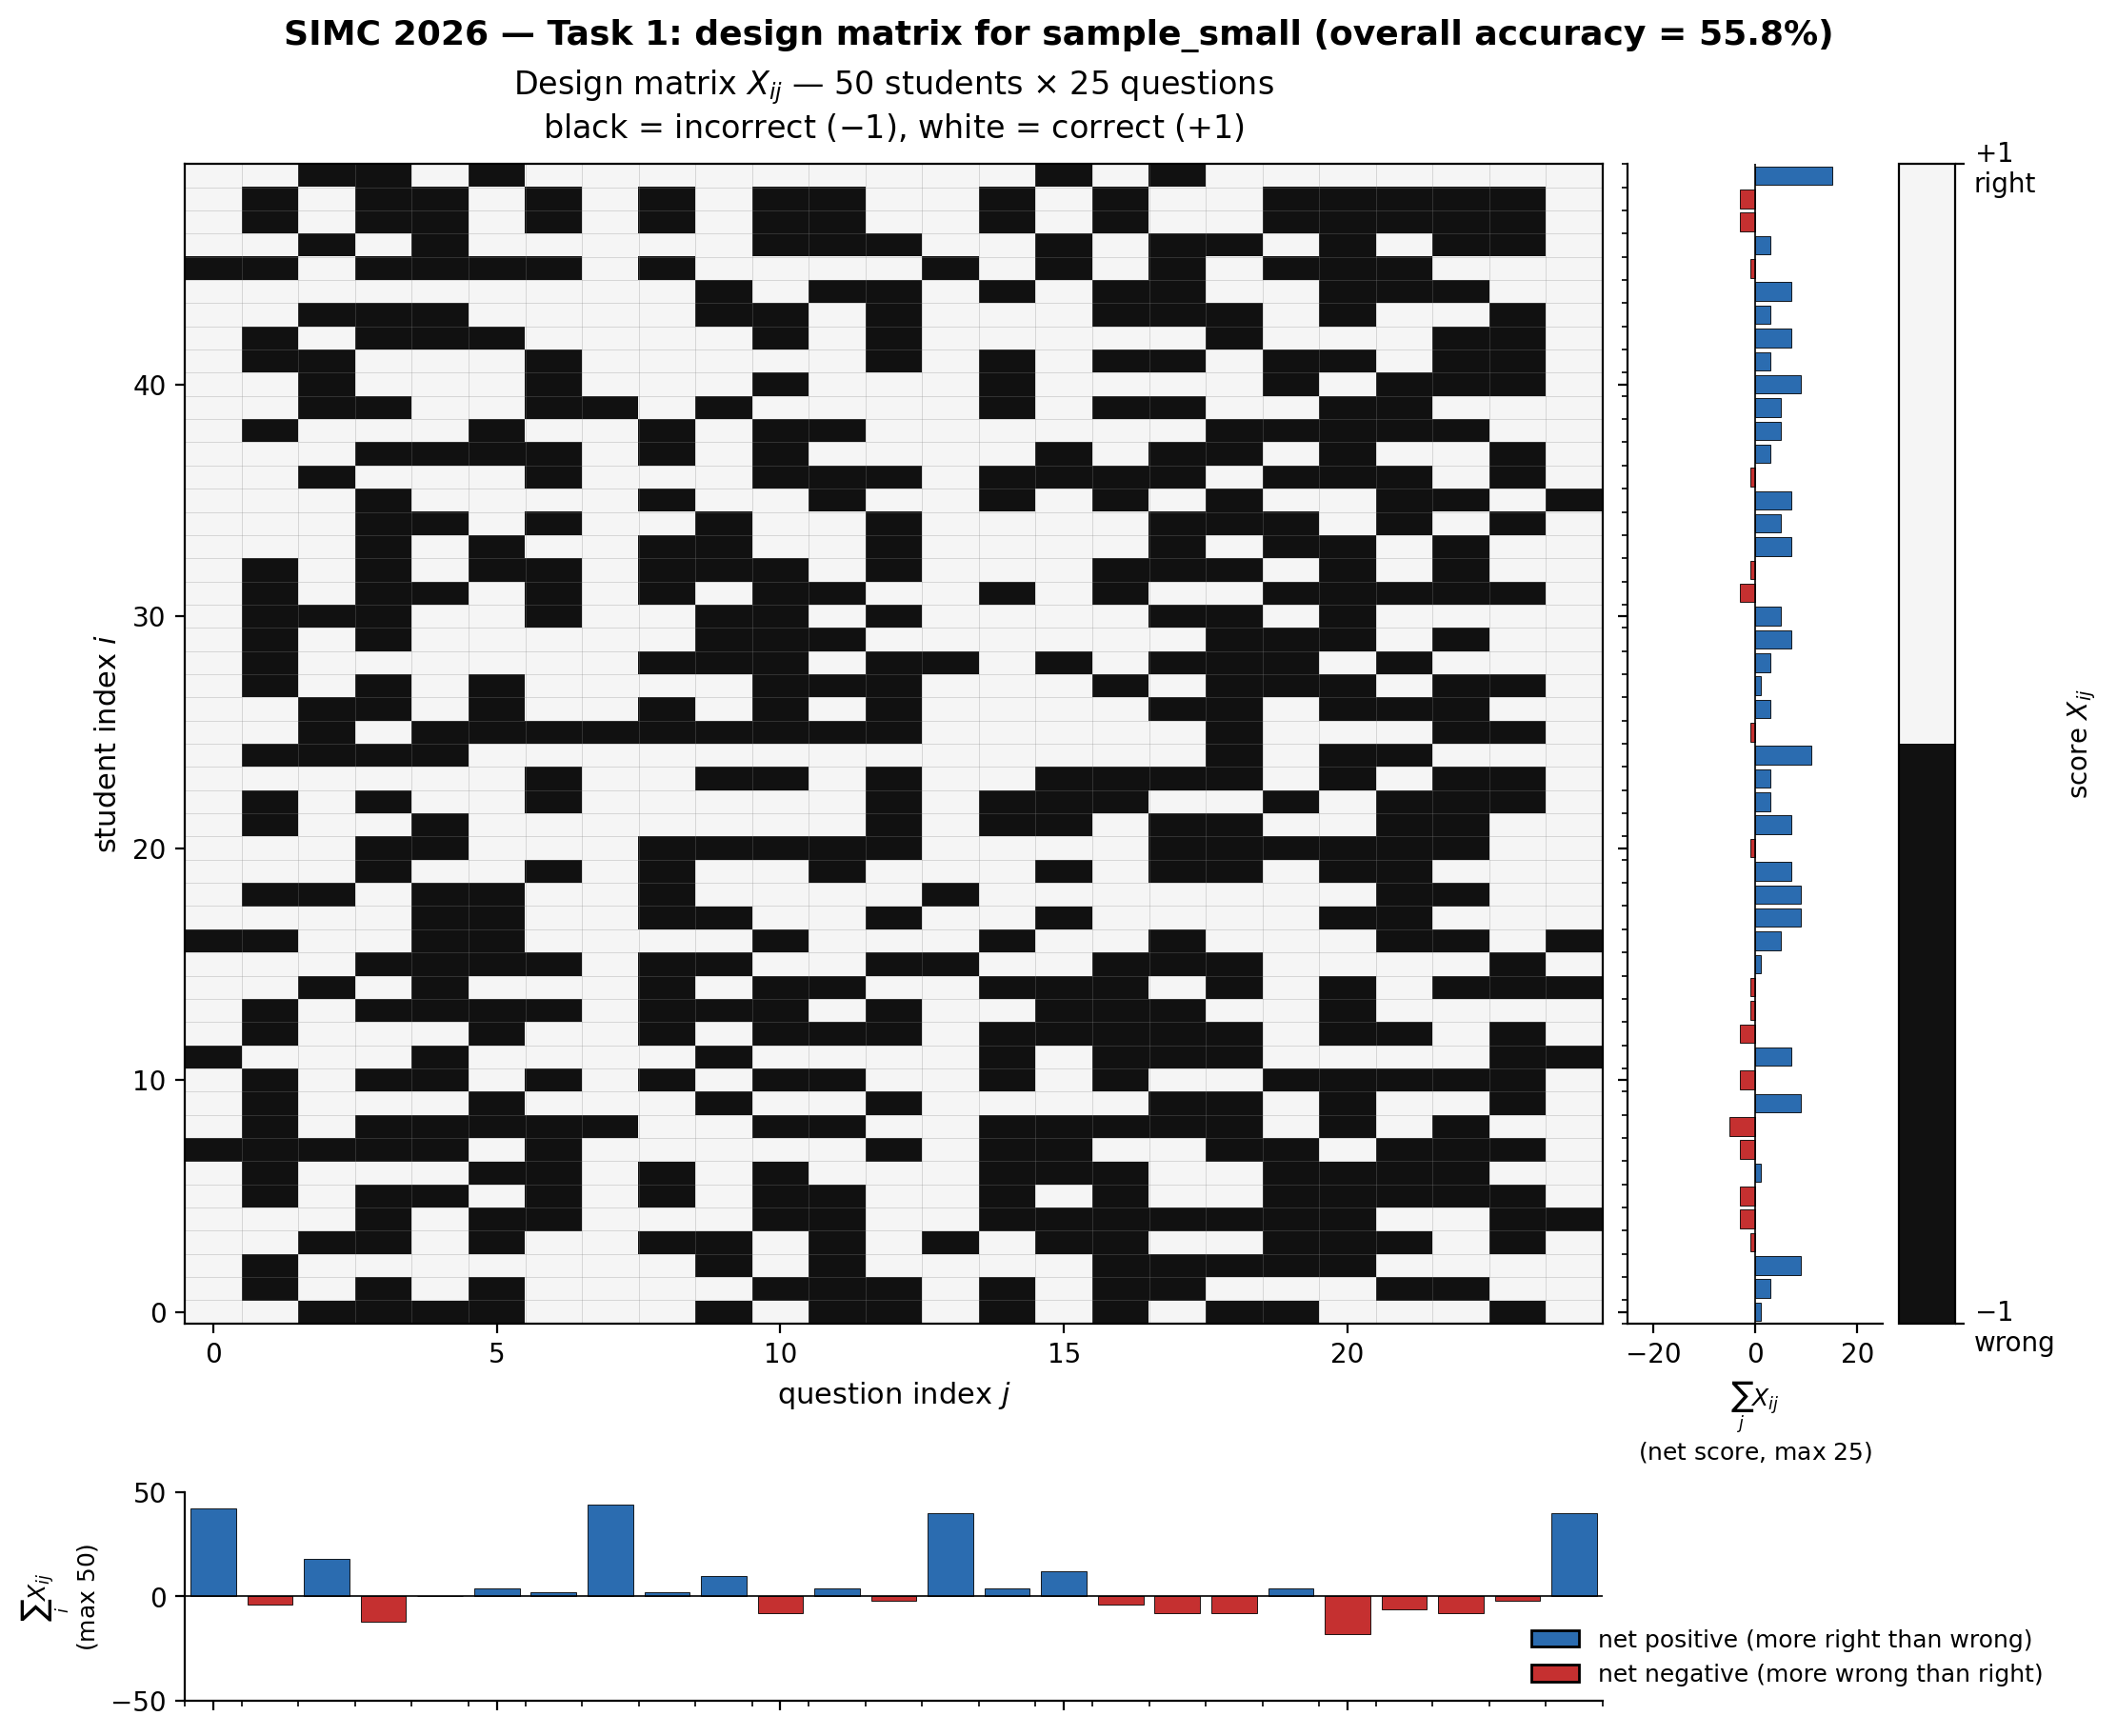
\includegraphics[width=0.95\linewidth]{../data/output/task1/task1_design_matrix.png}
  \caption{Design matrix for \texttt{sample\_small} ($M=50$, $N=25$).
  Black cells encode wrong answers, white cells encode correct answers.
  Right margin: student net scores. Bottom margin: question net scores.
  Overall accuracy is \SI{55.8}{\percent}.}
  \label{fig:task1}
\end{figure}

\begin{insight}[What the marginals already tell us]
The per-question bars expose a markedly uneven test: questions
$0$, $7$ and $23$ behave like ``free'' questions (net positive $> +35$),
while questions $19$--$22$ are net negative. \emph{Question difficulty is
not uniform.} Task~8 will exploit exactly this fact by estimating
per-question $p_j$ from column means before applying the null model.
\end{insight}

% ==================================================================
\section{Task 2 -- The Similarity Matrix}
% ==================================================================

\subsection{Construction}
Define the \emph{pairwise similarity matrix} $\Sm \in \mathbb{Z}^{M\times M}$
by
\begin{equation}
  S_{ij} \;\equiv\; (\X\X^{\!\top})_{ij}
         \;=\; \sum_{k=1}^{N} X_{ik}\,X_{jk}.
  \label{eq:sim}
\end{equation}
Because each factor is $\pm 1$, the contribution of question $k$ to
$S_{ij}$ is
\begin{equation}
  X_{ik}X_{jk} \;=\;
  \begin{cases}
    +1, & \text{students $i$ and $j$ \textbf{agreed} on question $k$,}\\
    -1, & \text{students $i$ and $j$ \textbf{disagreed} on question $k$.}
  \end{cases}
  \label{eq:sim-term}
\end{equation}
Consequently
\begin{equation}
  S_{ij} \;=\; \#\text{agreements} \;-\; \#\text{disagreements}
         \;\in\; \{-N,-N+2,\ldots,N\},
\end{equation}
with the diagonal pinned at $S_{ii} = N$ by construction (a student
always agrees with themselves on every question).

\subsection{Geometric interpretation}
Each row $\X_{i,\cdot}$ has constant Euclidean norm $\lVert\X_{i,\cdot}\rVert
= \sqrt{N}$, so $\Sm$ is, up to a constant, a \emph{cosine similarity}
matrix:
\begin{equation}
  \cos\theta_{ij}
  \;=\; \frac{\langle\X_{i,\cdot},\X_{j,\cdot}\rangle}
             {\lVert\X_{i,\cdot}\rVert\,\lVert\X_{j,\cdot}\rVert}
  \;=\; \frac{S_{ij}}{N}.
  \label{eq:cos}
\end{equation}
This is the key bridge to clustering algorithms (Task~3): \emph{any}
distance-based clustering on the rows of $\X$ implicitly partitions
students by cosine similarity, i.e.\ by $\Sm$.

\subsection{Visualisation and outliers}
Figure~\ref{fig:task2} plots $\Sm$ as a diverging heatmap together with
the histogram of all $\binom{M}{2} = 1225$ unique off-diagonal entries.

\begin{figure}[htb]
  \centering
  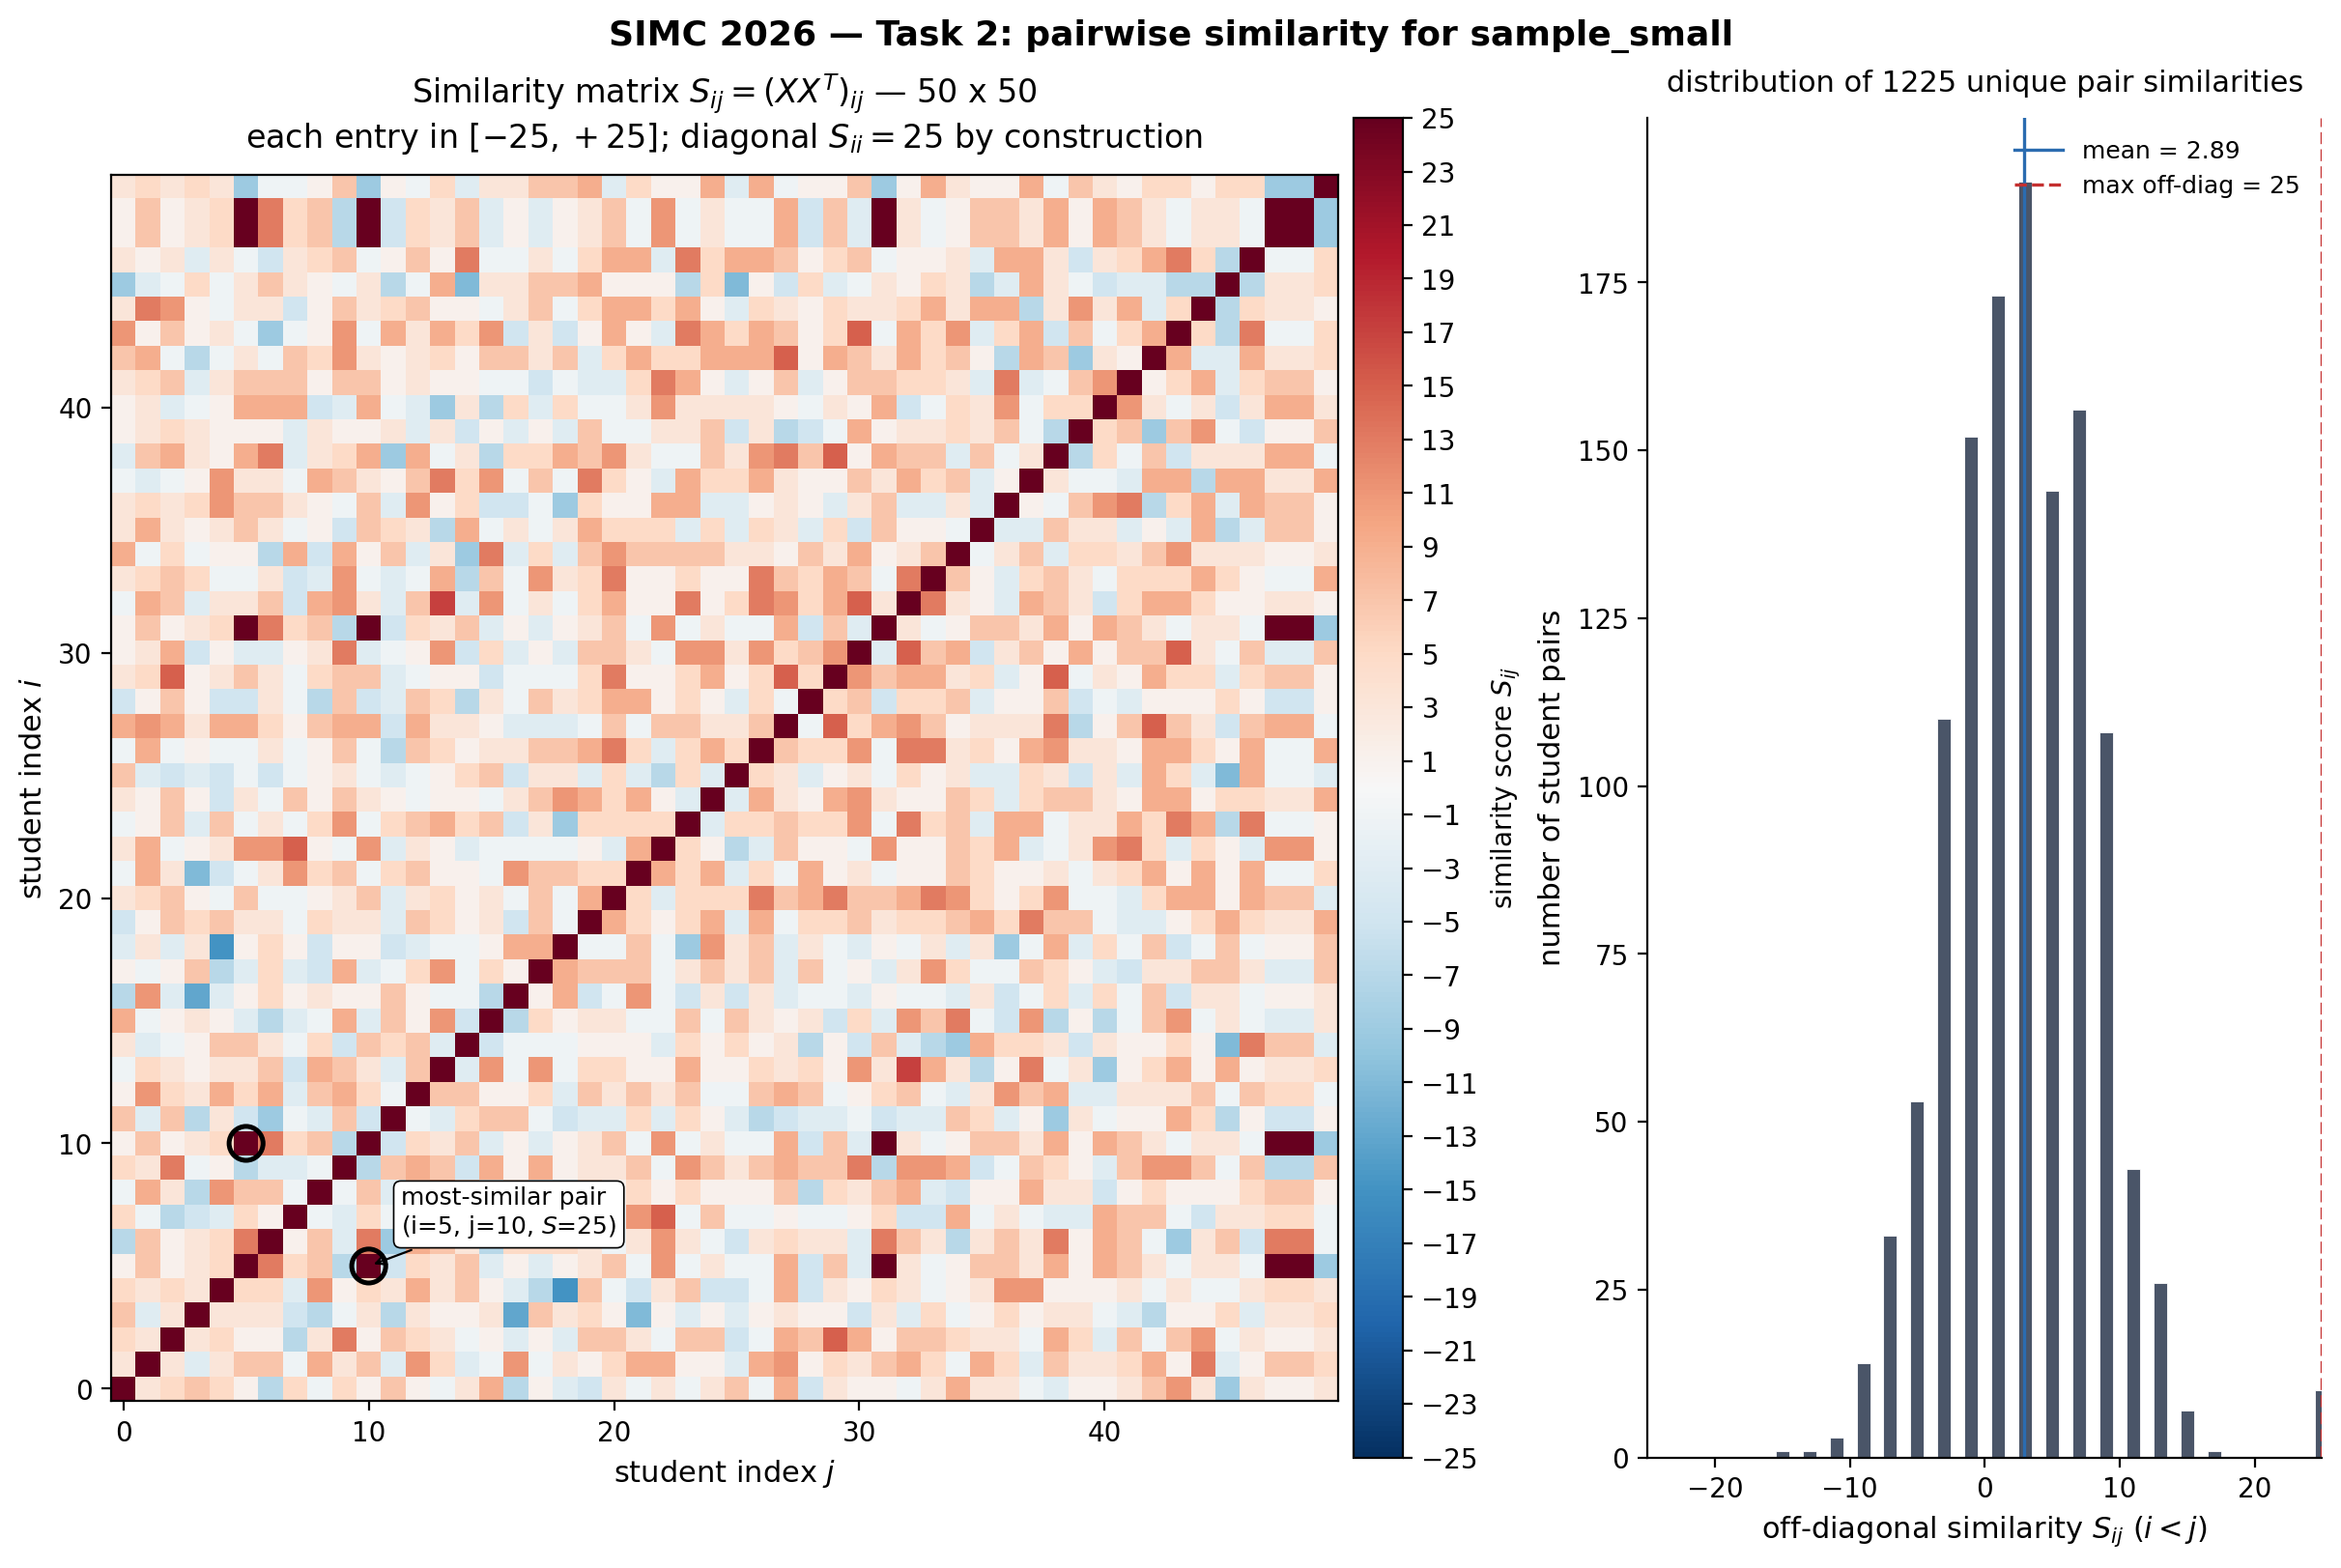
\includegraphics[width=0.95\linewidth]{../data/output/task2/task2_similarity_matrix.png}
  \caption{Left: similarity matrix $\Sm = \X\X^{\!\top}$ for
  \texttt{sample\_small}. The diagonal $S_{ii}=N=25$ is dark red.
  Right: histogram of off-diagonal $S_{ij}$ with $i<j$.}
  \label{fig:task2}
\end{figure}

\begin{keyresult}[A single pair sits at the theoretical maximum]
The maximum off-diagonal similarity is $S_{5,10} = 25 = N$, meaning
students $5$ and $10$ \textbf{agreed on all 25 questions}. The bulk of
the histogram has mean $\bar S_{\text{off}} \approx 2.89$ with a roughly
Gaussian spread, so the $(5,10)$ entry is a striking outlier in the
right tail.
\end{keyresult}

% ==================================================================
\section{Task 3 -- Clustering with $K$-means and Silhouette Analysis}
% ==================================================================

\subsection{Algorithm}
$K$-means partitions $\{\X_{i,\cdot}\}_{i=1}^{M}$ into $K$ disjoint
groups by alternately
\begin{enumerate}[label=(\alph*),leftmargin=2.2em]
  \item assigning each student to the cluster whose centroid is
        closest, and
  \item recomputing centroids as the mean of their assigned members,
\end{enumerate}
until centroids stabilise. To mitigate sensitivity to the random
initial centroids we use scikit-learn's \texttt{n\_init=20}.

\subsection{Visualising cluster quality}
For each $K$ we render $\Sm$ with its rows and columns permuted by
cluster label. A good $K$ produces solid red squares on the diagonal
(in-group agreement) against a paler background (out-group
disagreement). Figure~\ref{fig:task3-sweep} shows three representative
values.

\begin{figure}[htb]
  \centering
  \begin{subfigure}[t]{0.32\linewidth}
    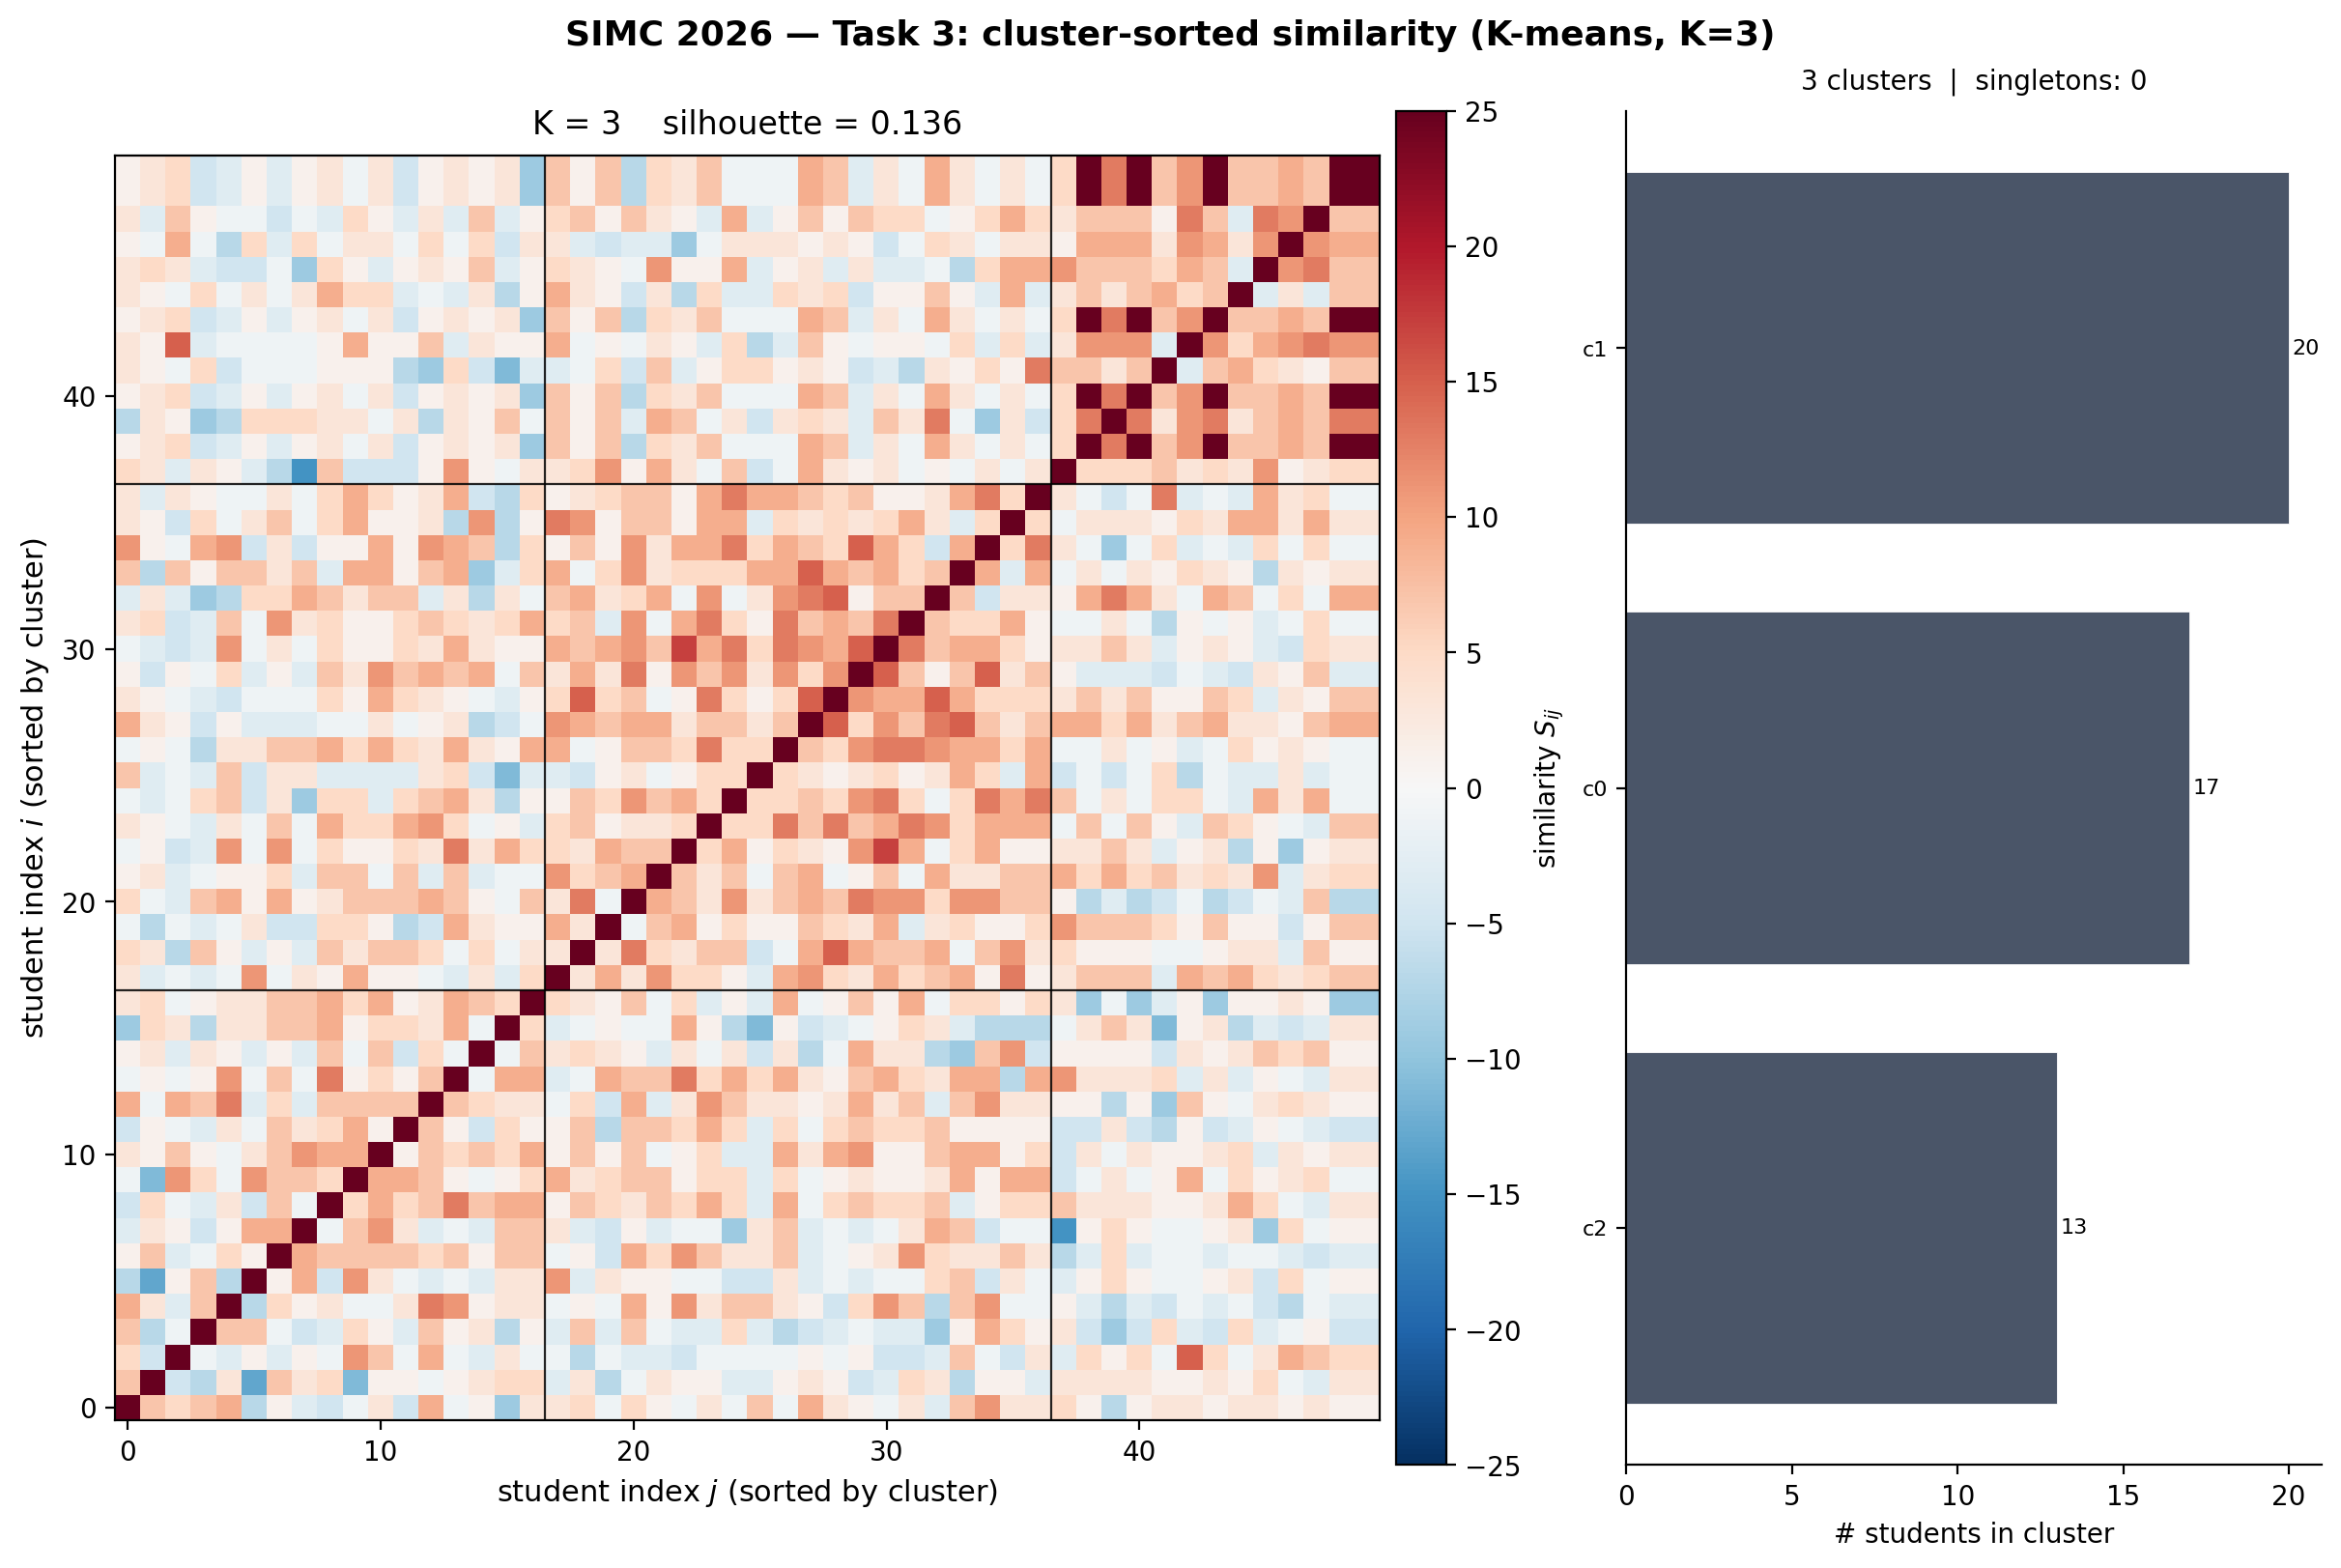
\includegraphics[width=\linewidth]{../data/output/task3/task3_similarity_K03.png}
    \caption{$K=3$: too few; visible block structure is coarse.}
  \end{subfigure}\hfill
  \begin{subfigure}[t]{0.32\linewidth}
    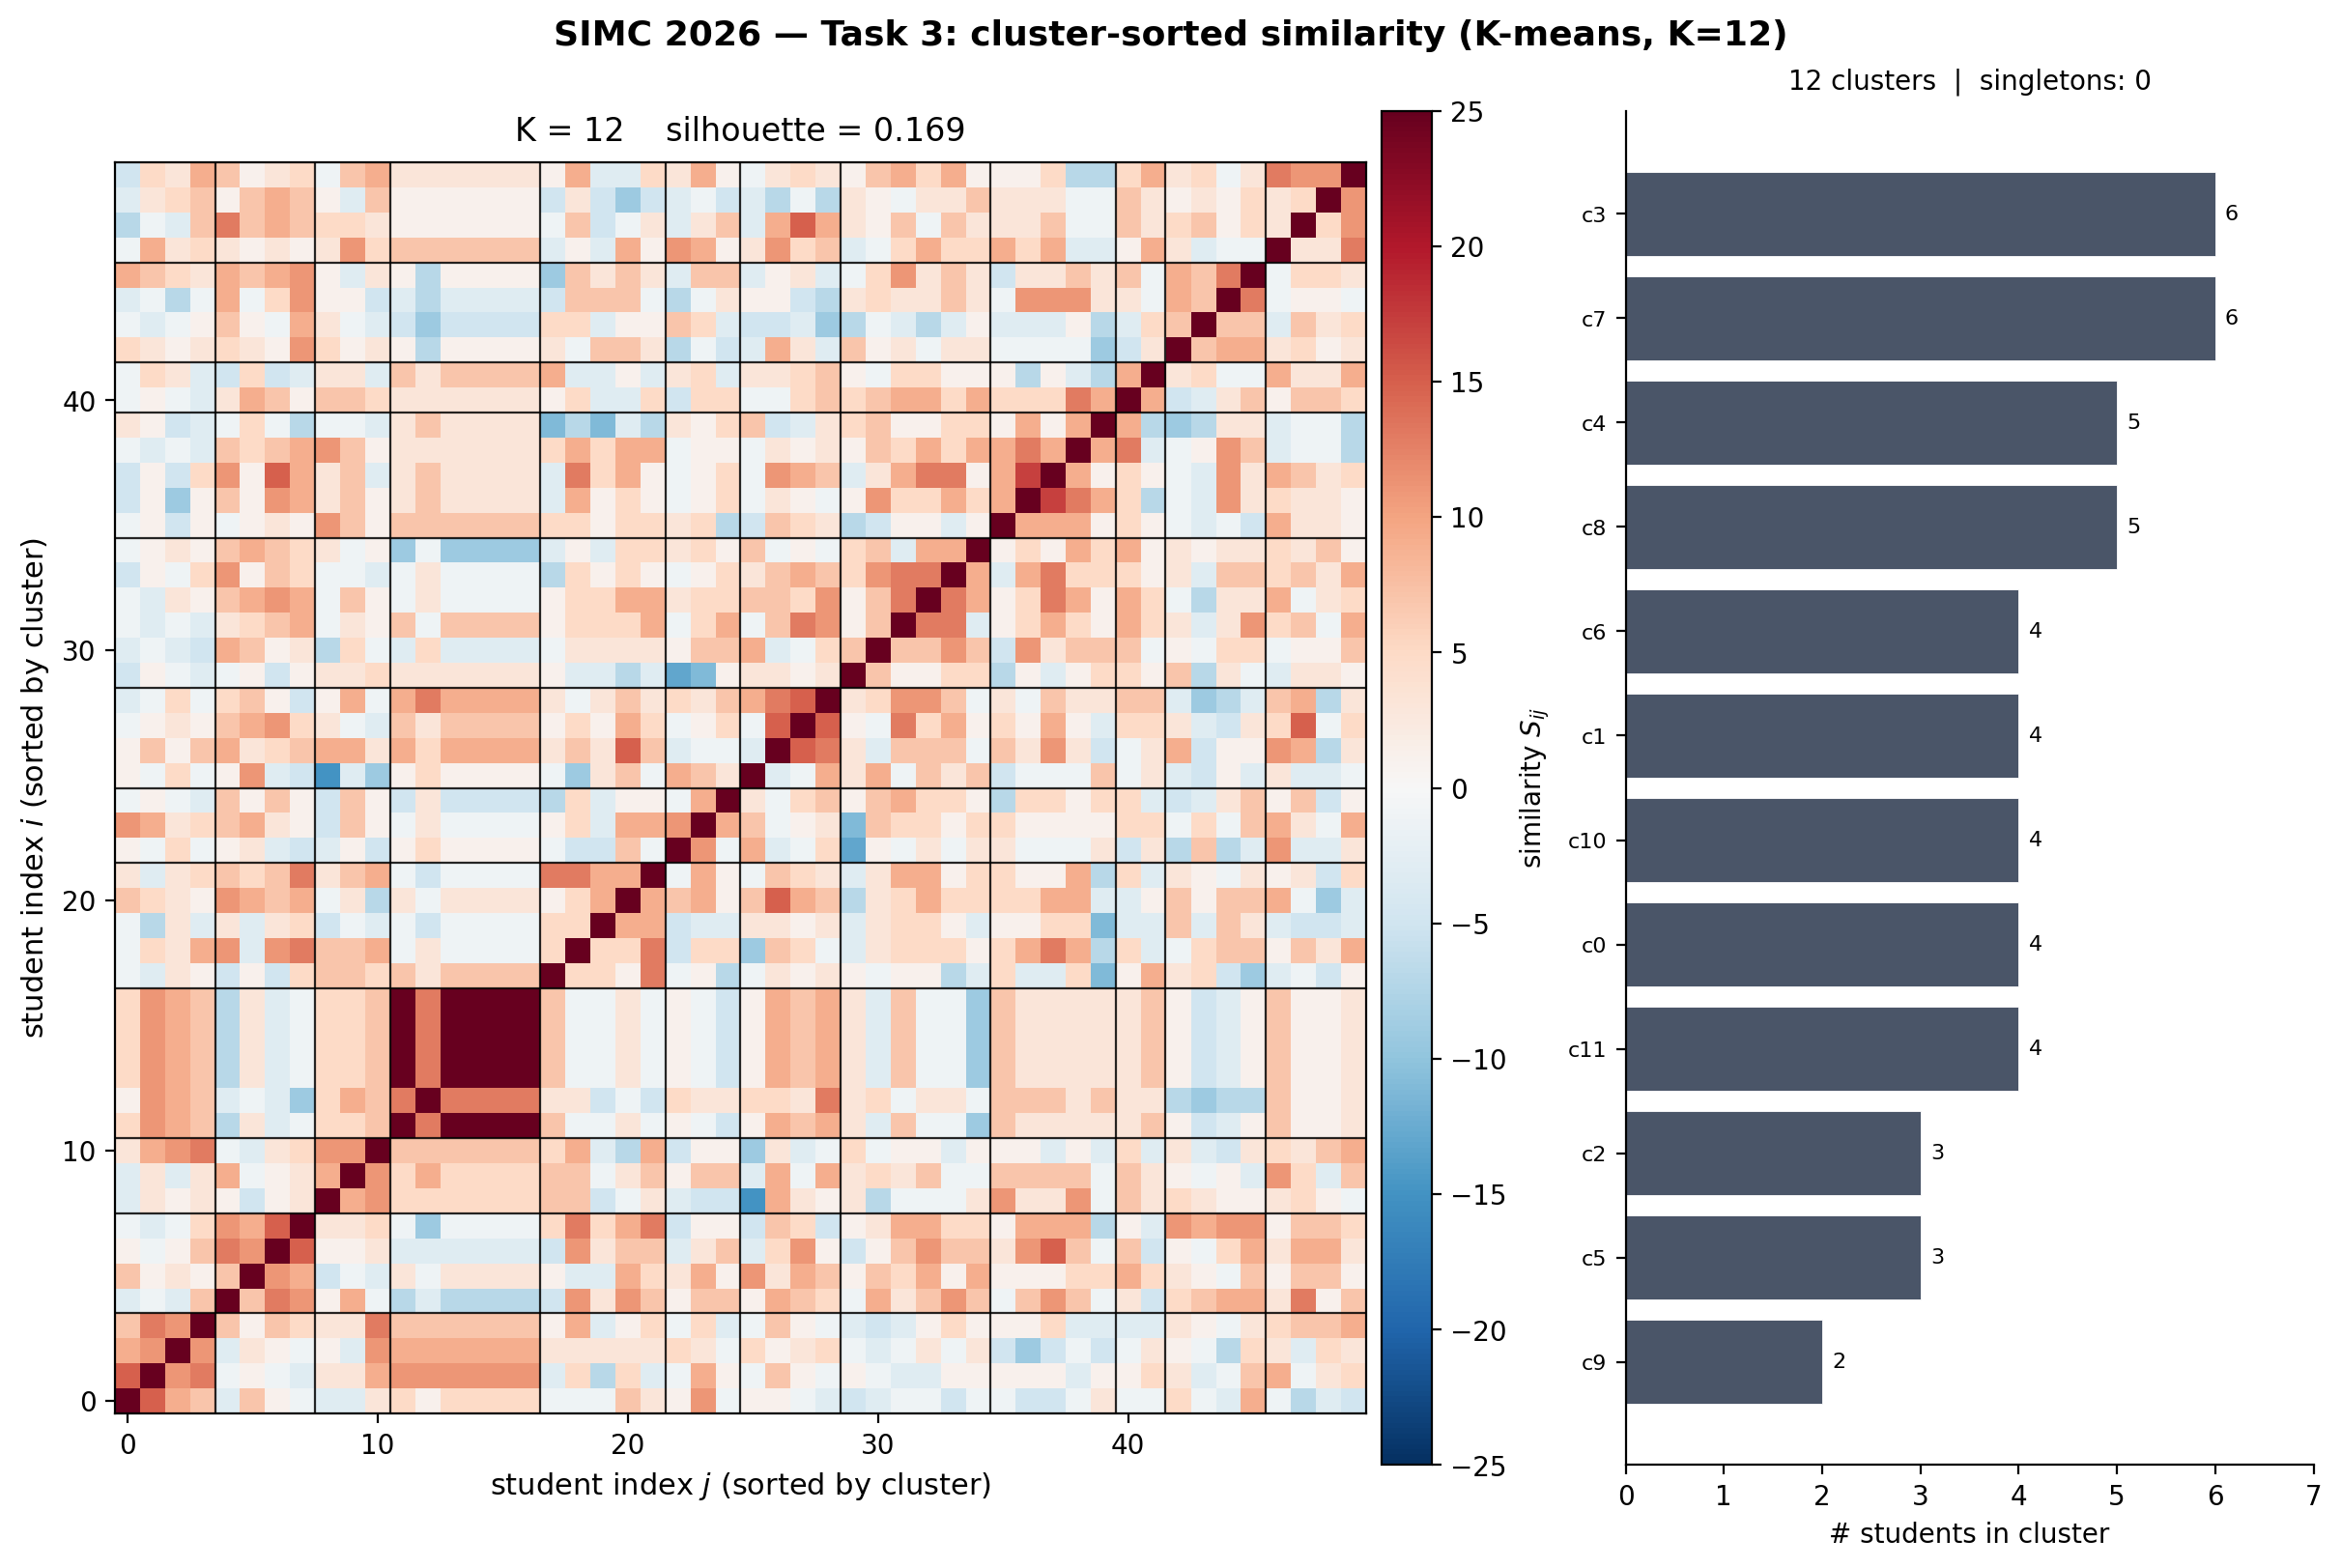
\includegraphics[width=\linewidth]{../data/output/task3/task3_similarity_K12.png}
    \caption{$K=12$: clean diagonal blocks, no singletons.}
  \end{subfigure}\hfill
  \begin{subfigure}[t]{0.32\linewidth}
    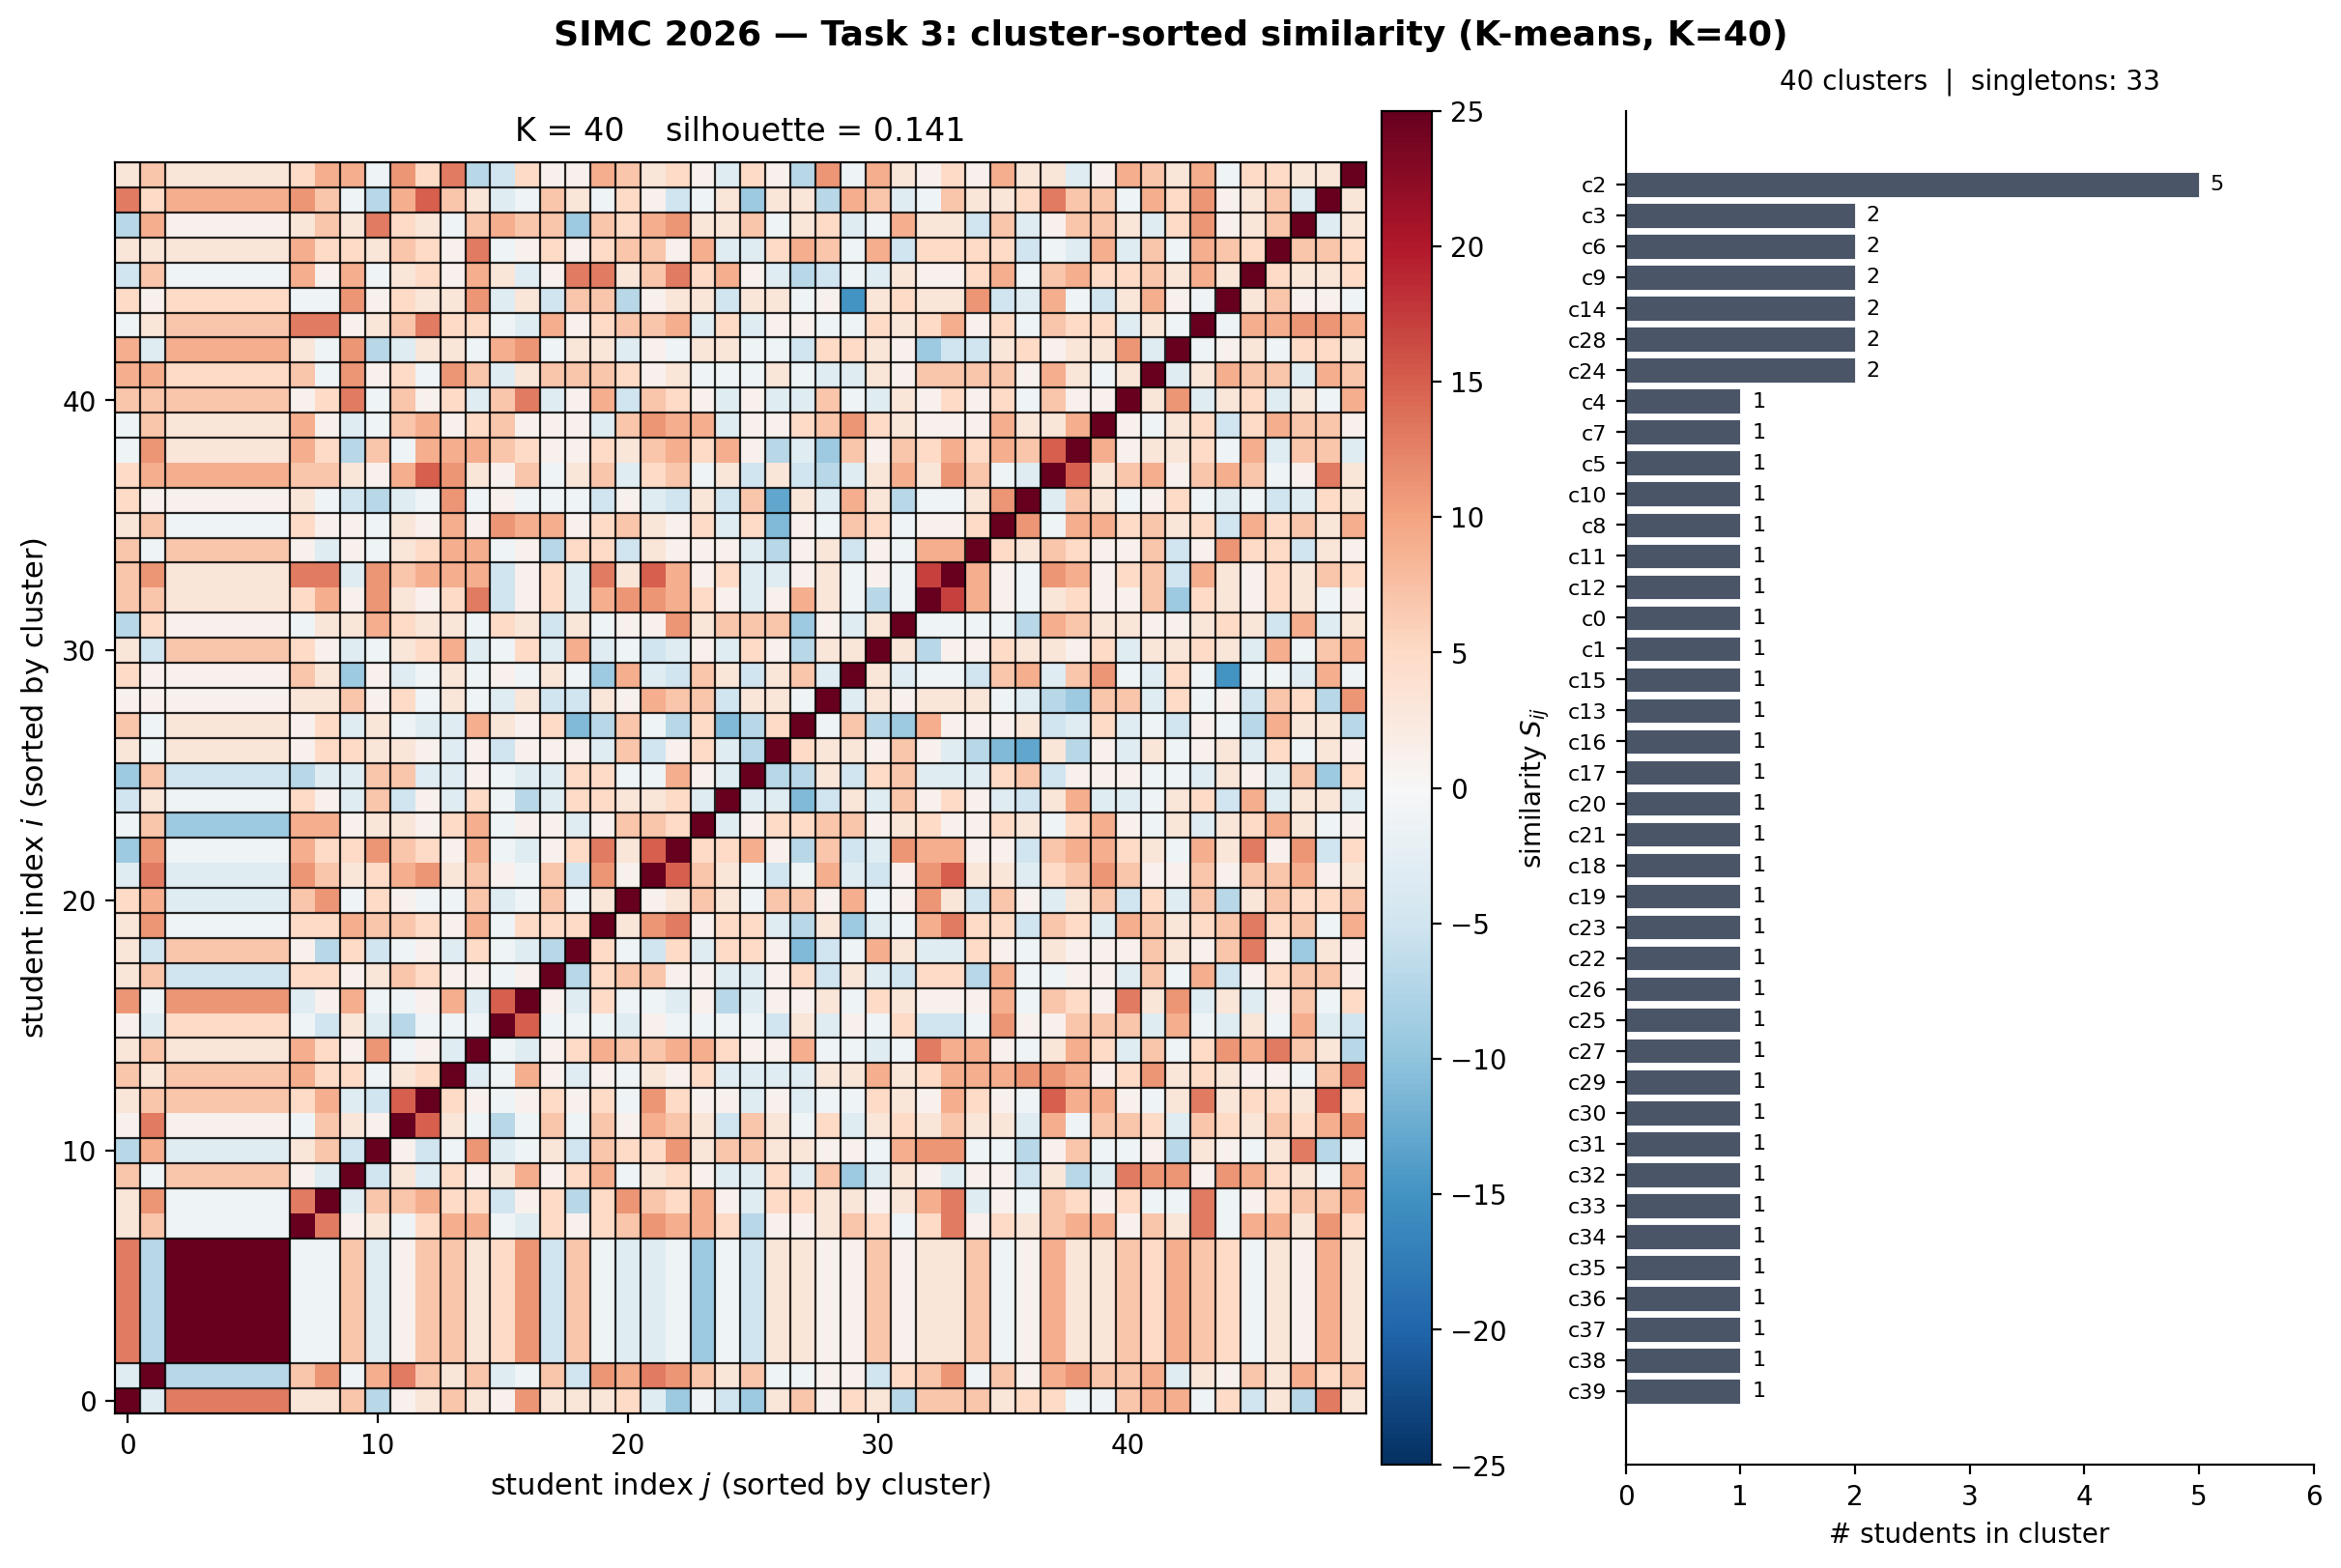
\includegraphics[width=\linewidth]{../data/output/task3/task3_similarity_K40.png}
    \caption{$K=40$: severely fragmented (33 singleton clusters).}
  \end{subfigure}
  \caption{Cluster-sorted similarity matrices for three values of $K$.}
  \label{fig:task3-sweep}
\end{figure}

\subsection{Silhouette score}
For a single point $i$ assigned to cluster $C(i)$, let $a(i)$ be its
mean (cosine) distance to other in-cluster points and
$b(i)=\min_{C\neq C(i)}\bar d(i,C)$ its mean distance to the nearest
\emph{foreign} cluster. The silhouette is
\begin{equation}
  s(i) \;=\; \frac{b(i)-a(i)}{\max\{a(i),b(i)\}}\;\in\;[-1,1],
  \qquad
  \mathrm{Silh}(K) \;=\; \frac{1}{M}\sum_{i=1}^{M} s(i).
  \label{eq:silh}
\end{equation}
Because our rows have constant norm, the natural distance is
$d_{\cos}(i,j) = 1 - S_{ij}/N$ -- the silhouette is computed in the same
geometry as $\Sm$ itself.

\subsection{The silhouette trap and our fix}
\label{sec:silh-trap}
A naive ``pick the $K$ that maximises $\mathrm{Silh}(K)$'' rule selects
$K^\star_{\text{raw}} = 30$ for our data, with
$\mathrm{Silh}(30) = 0.186$. But $K=30$ has \textbf{17 of 30 clusters
containing a single student}, the very pathology the problem statement
flags as ``defeating the purpose of clustering''. The mechanism is
mechanical:

\begin{insight}[Why silhouette over-rewards singletons]
A singleton cluster has $a(i)$ \emph{undefined} and the convention sets
$s(i)=0$, but every \emph{non-singleton} member of any other cluster
gains a more distant ``nearest foreign cluster'' as singletons are
peeled off, inflating their $b(i)$. The aggregate
$\mathrm{Silh}(K)$ therefore tends to drift upward with $K$ even after
the partition has lost meaning.
\end{insight}

We therefore use a \textbf{singleton-filtered silhouette criterion}:
\begin{equation}
  K^\star \;=\; \arg\max_{K\;:\;\min_c |C_c|\,\geq\,2}\;\mathrm{Silh}(K).
  \label{eq:filter}
\end{equation}
Table~\ref{tab:silh} summarises the sweep.

\begin{table}[htb]
  \centering
  \begin{tabular}{r r r l}
    \toprule
    $K$ & $\mathrm{Silh}(K)$ & \#\,singletons & eligible? \\
    \midrule
    2   & 0.166 & 0  & \checkmark \\
    3   & 0.136 & 0  & \checkmark \\
    5   & 0.136 & 0  & \checkmark \\
    8   & 0.147 & 0  & \checkmark \\
    \textbf{10}  & \textbf{0.169} & \textbf{0}  & \textbf{\checkmark\ (winner)} \\
    12  & 0.169 & 0  & \checkmark \\
    15  & 0.177 & 2  & $\times$ \\
    20  & 0.171 & 6  & $\times$ \\
    25  & 0.183 & 10 & $\times$ \\
    30  & 0.186 & 17 & $\times$ \\
    40  & 0.141 & 33 & $\times$ \\
    \bottomrule
  \end{tabular}
  \caption{Silhouette sweep on \texttt{sample\_small}. Raw silhouette
  peaks at $K=30$, but Eq.~\eqref{eq:filter} disqualifies it.}
  \label{tab:silh}
\end{table}

\begin{figure}[htb]
  \centering
  \begin{subfigure}[t]{0.55\linewidth}
    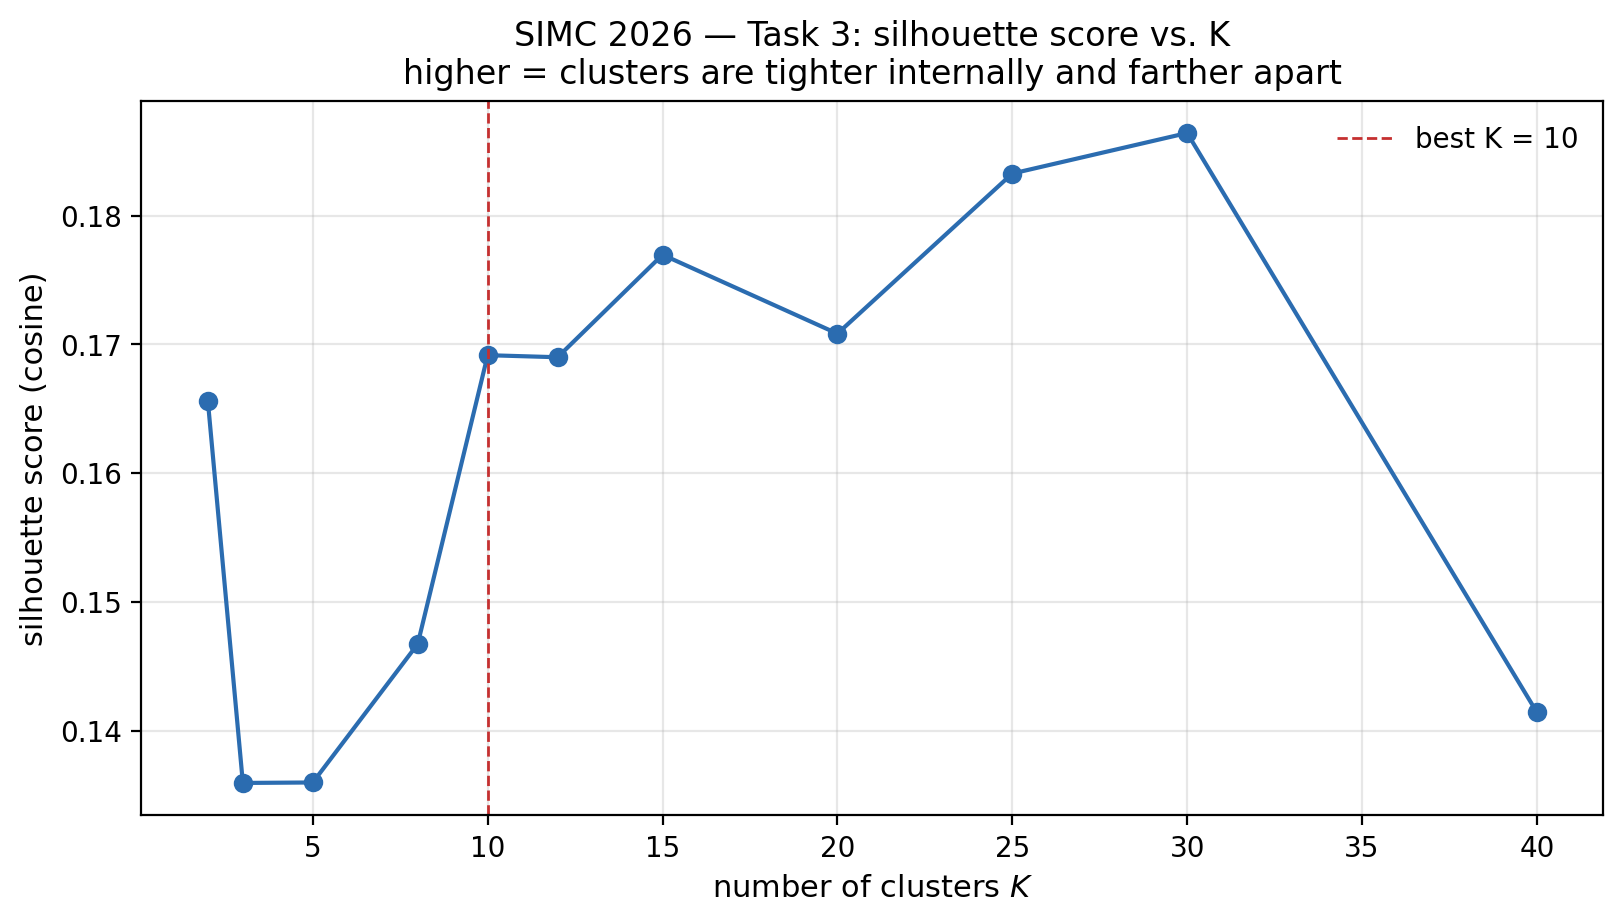
\includegraphics[width=\linewidth]{../data/output/task3/task3_silhouette_curve.png}
  \end{subfigure}
  \begin{subfigure}[t]{0.42\linewidth}
    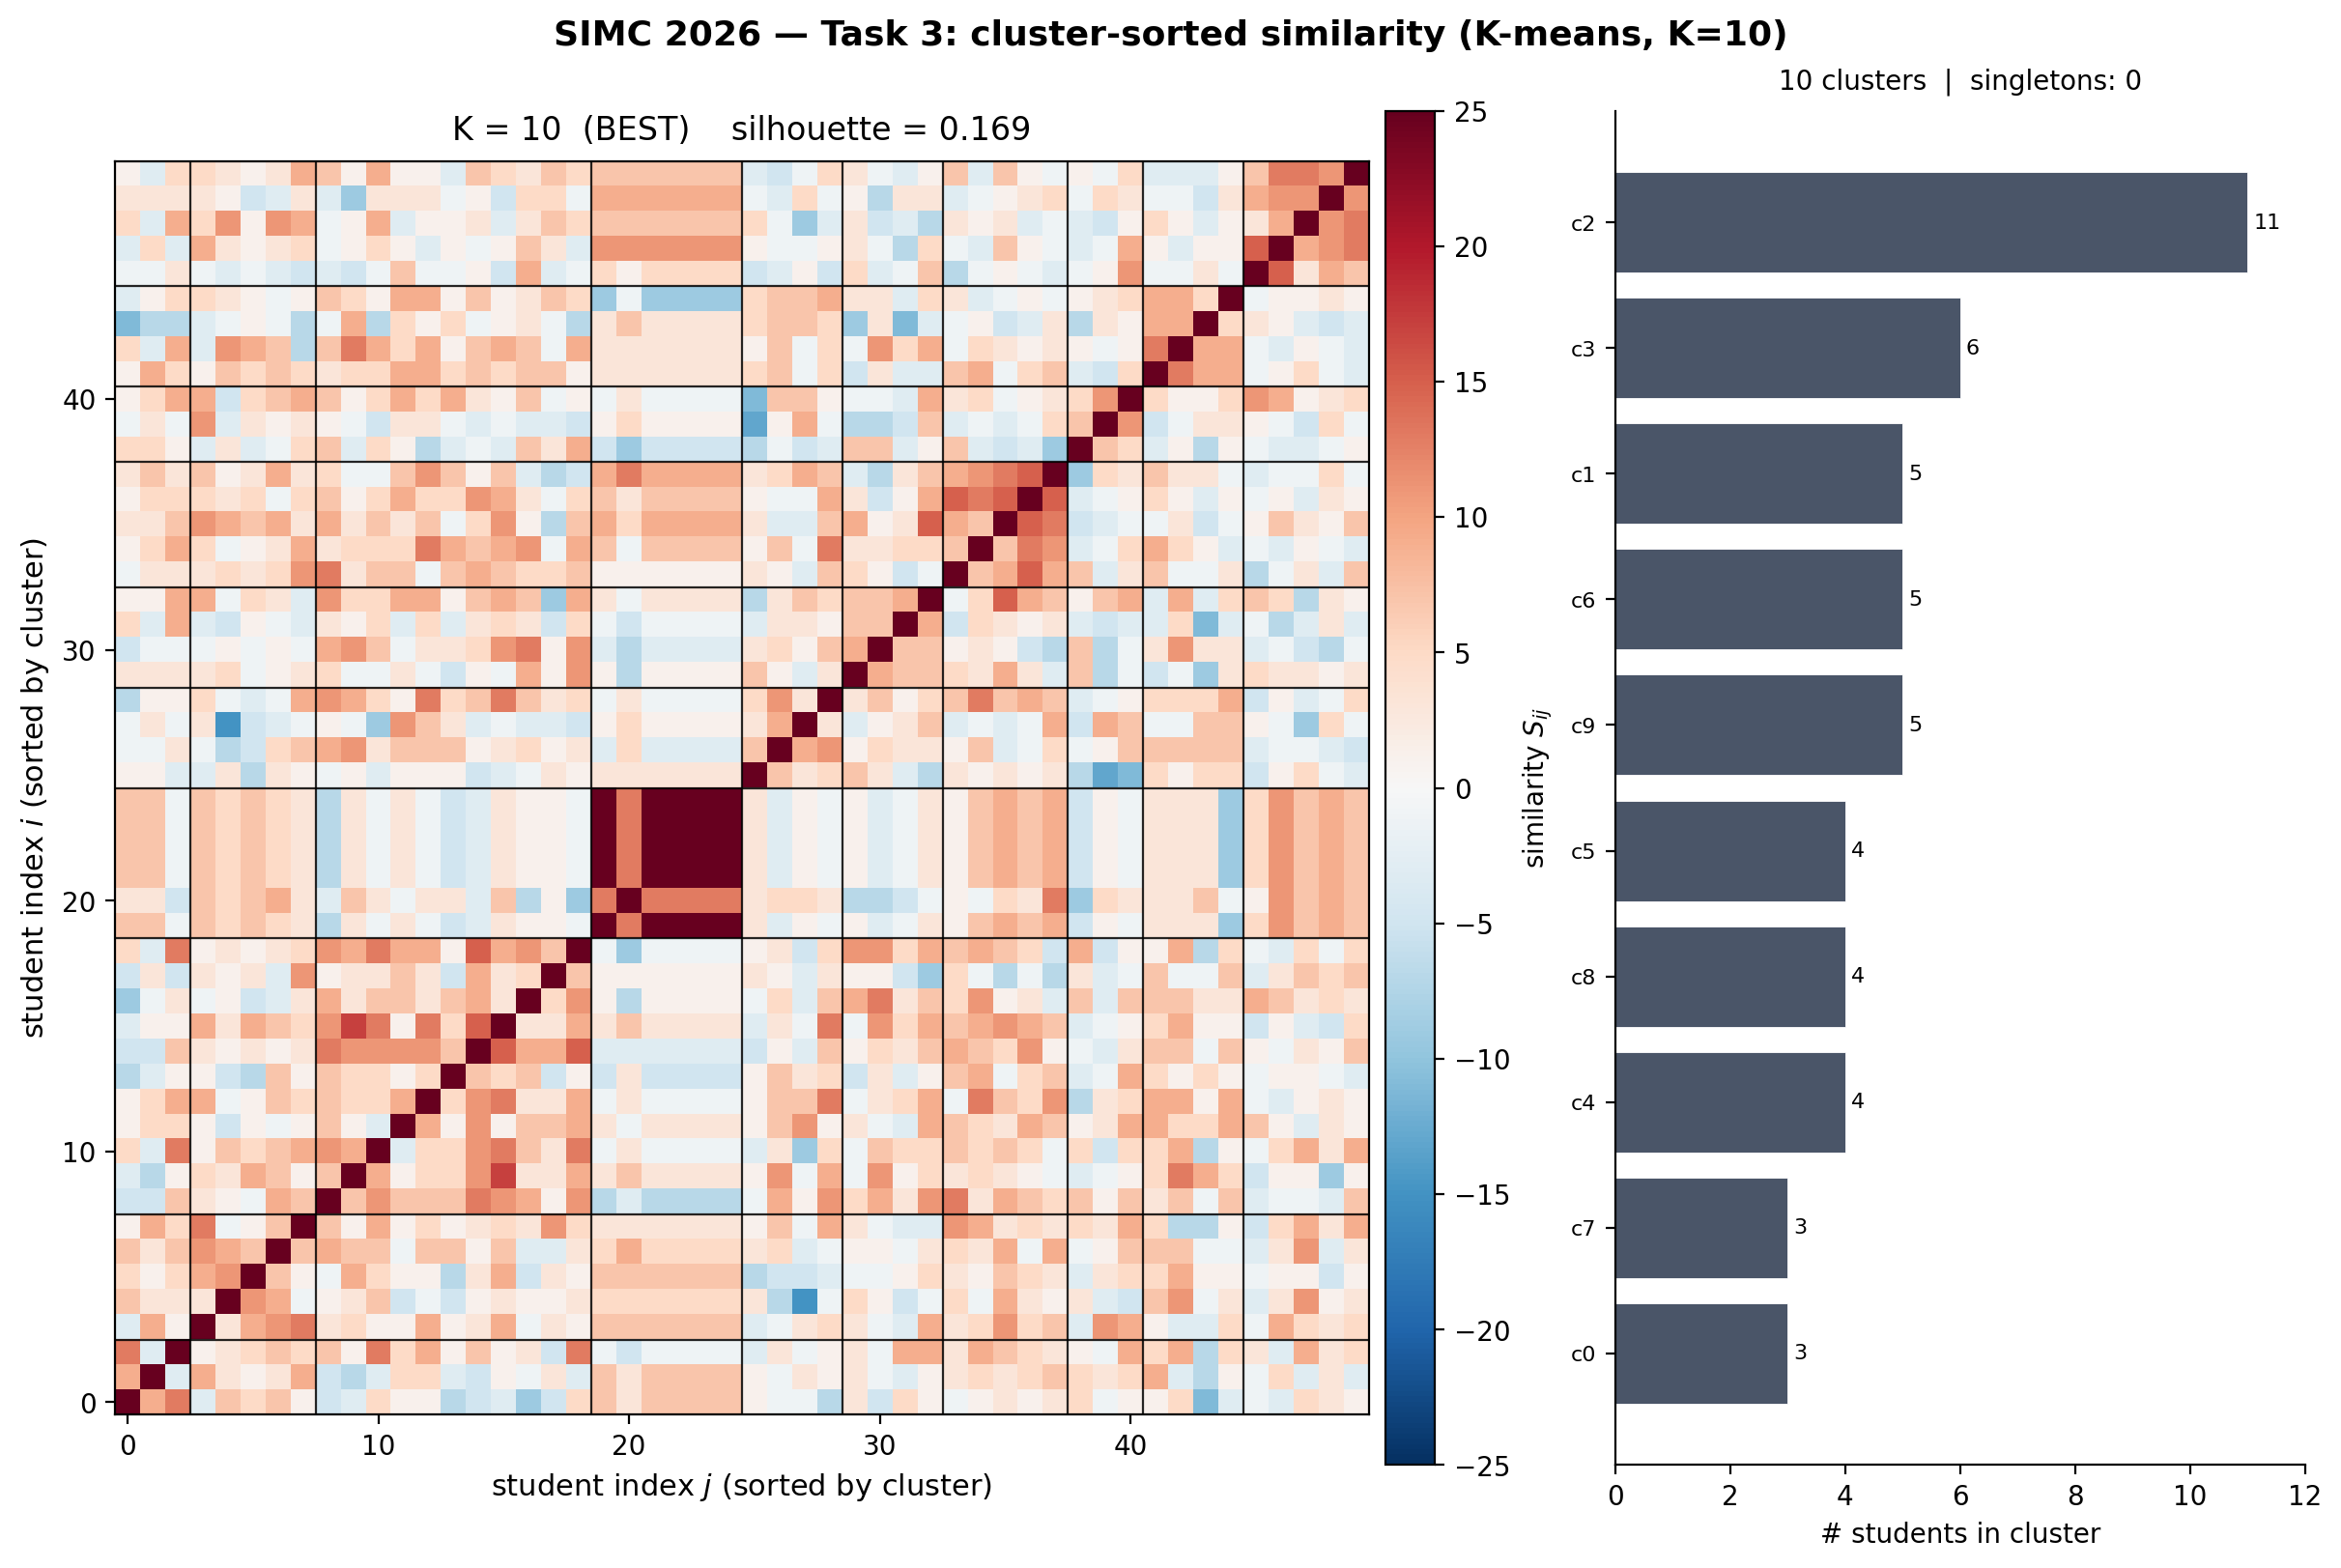
\includegraphics[width=\linewidth]{../data/output/task3/similarity_best_task3.png}
  \end{subfigure}
  \caption{Left: silhouette as a function of $K$. Right: best
  cluster-sorted similarity matrix at $K^\star = 10$.}
  \label{fig:task3-best}
\end{figure}

\begin{keyresult}[Selected partition]
The singleton-filtered criterion selects $K^\star = 10$ with
$\mathrm{Silh} = 0.169$. Cluster sizes range from $3$ to $11$ students,
and the cluster containing students $5$ and $10$ is the deepest red
block on the diagonal -- a clustering-level corroboration of the
collusion candidate found in Task~2.
\end{keyresult}

% ==================================================================
\section{Task 4 -- A Plausibility Argument for Collusion}
% ==================================================================

\subsection{Can we already name names? Honestly, no.}
Tasks~1--3 give us a heatmap, a Gram matrix, and a partition into
$K^\star = 10$ clusters. None of these tools is a \emph{detector} of
cheating. The design matrix tells us only \emph{what} each student
answered; it does not tell us \emph{how} they came to that answer.
Two students might score identically because:
\begin{enumerate}[leftmargin=2em,nosep]
  \item one copied from the other;
  \item they prepared together from the same notes and learned the same
        gaps;
  \item they happen to be of similar ability on similar topics; or
  \item pure luck on a short test.
\end{enumerate}
Without a probability model we cannot rank these explanations against
each other. So any sentence of the form \emph{``students $i$ and $j$
colluded''} is, at this stage, an overreach. The honest conclusion is
weaker but still useful: \emph{some pairs look unlike what we would
naively expect, and they deserve a closer look}.

\subsection{Shift the goal: suspects, not convicts}
A useful change of framing is to stop trying to convict anyone and
start trying to \emph{shortlist suspects}. The two tasks have very
different evidentiary requirements:
\begin{itemize}[leftmargin=2em,nosep]
  \item \textbf{Conviction} demands a low-error decision rule, e.g.\
        a calibrated $p$-value below some threshold. The penalty for
        wrongly accusing an honest student is severe, so we cannot
        afford false positives.
  \item \textbf{Suspect-flagging} only demands that the shortlist
        contains the truly suspicious pairs. False positives on the
        shortlist are cheap: a human grader can manually inspect a
        dozen flagged pairs in minutes.
\end{itemize}
For a class of $M = 50$ students there are $\binom{50}{2} = 1225$
distinct pairs -- far too many to review by hand. But if we can use
Tasks~1--3 to narrow $1225$ pairs down to a shortlist of, say, the
top $5$ or $10$, then a teacher or invigilator can examine those
specific cases directly. \textbf{We are doing triage, not jurisprudence.}
Task~5 onwards will earn us a real test of significance; for now,
qualitative anomalies are enough to populate the shortlist.

\subsection{Where would collusion ``leak'' into our analysis?}
Even without a null model, three independent fingerprints in our
existing analyses point toward the same suspect pair, and all three
are the \emph{kind} of pattern we would expect collusion to leave
behind.

\paragraph{Fingerprint 1 -- impossibly perfect agreement on a non-trivial
test.} The pair $(i,j) = (5,10)$ has $S_{5,10} = +25$. Because
$S_{ij} = N - 2\cdot(\#\text{disagreements})$, this is only possible
when the two students disagree on \emph{zero} questions. On a uniform
test where every answer is a coin flip, the chance of zero
disagreements over $N$ questions is $\bigl(\tfrac12\bigr)^N$ -- already
$1/3.4\times 10^7$ for $N=25$. Realistic tests have some easy
questions where two honest students naturally agree, which raises the
probability, but the qualitative point survives: \emph{perfect
agreement is the regime where coincidence runs out of room}.

\paragraph{Fingerprint 2 -- agreement on the \emph{hard} questions as
well as the easy ones.} Figure~\ref{fig:task1} shows that question
difficulty in this test is markedly non-uniform: questions $0$, $7$,
$23$ are nearly-free (large positive column sums) while questions
$19$--$22$ are net-negative (most students get them wrong). Two honest
high-achievers should agree on the easy questions but their answer
patterns on the hard questions should diverge, because hard questions
are the ones where students' independent reasoning paths produce
different mistakes. Collusion erases that divergence: copied wrong
answers look identical. The fact that students $5$ and $10$ agree on
\emph{every} question, easy and hard alike, is the
``honest-students-shouldn't-look-like-this'' signature.

\paragraph{Fingerprint 3 -- crystalline cluster co-membership.} Honest
similarity is \emph{fuzzy}: as we sweep $K$ in $K$-means, an honest
pair's cluster co-membership flickers on and off depending on how the
boundaries are drawn. A colluding pair, by contrast, has effectively
identical feature vectors, so they sit on top of each other in feature
space and remain co-clustered \emph{across every choice of $K$}. In
our sweep $K \in \{2,3,5,8,10,12,15,20,25,30,40\}$, students $5$ and
$10$ never separated. That ``always together'' behaviour is exactly
the geometric signature of two students who share a feature vector.

\subsection{The data behind the shortlist}
Combining the empirical similarity distribution from Task~2 with the
clustering output from Task~3 gives Table~\ref{tab:suspects}, our
working suspect shortlist for \texttt{sample\_small}.

\begin{table}[htb]
  \centering
  \begin{tabular}{c c c c l}
    \toprule
    pair $(i,j)$ & $S_{ij}$ & $(S_{ij}-\bar S)/\hat\sigma$ &
        always co-clustered? & verdict \\
    \midrule
    $(5,10)$ & $25$ & $\approx +3.5$ & yes ($K=2$--$40$) & \textbf{strong suspect} \\
    \multicolumn{5}{c}{\emph{empirical baseline}}\\
    all $1225$ pairs & --- & --- & --- &
        $\bar S \approx 2.89$, $\hat\sigma \approx 6.3$ \\
    diagonal $S_{ii}$ & $25$ & --- & trivially & not informative \\
    \bottomrule
  \end{tabular}
  \caption{Suspect shortlist after Tasks~1--3. Only one off-diagonal
  pair $(5,10)$ stands clearly above the empirical noise floor.
  $\bar S$ and $\hat\sigma$ are computed on the $1225$ unique
  upper-triangular off-diagonal entries of $\Sm$.}
  \label{tab:suspects}
\end{table}

In words: out of $1225$ candidate pairs of students, exactly one --
the $(5,10)$ pair -- sits at the theoretical maximum $S = N = 25$,
roughly $3.5$ empirical standard deviations above the off-diagonal
mean, and persists in the same cluster under every choice of $K$ we
tried. \textbf{That one pair is our suspect.} Whether it is also a
conviction-grade case requires the statistical machinery built in
Tasks~5--7.

\begin{insight}[Hint from the problem statement]
The problem explicitly warns ``you might not actually get too far''
without a statistical null model. Our reading is sharper: we can
\emph{shortlist} (we just did), but we cannot \emph{prove}. The proof
step -- attaching a probability to the observed $S = 25$ -- is
exactly what Task~5 sets up by deriving the null-model mean and
standard deviation, which Tasks~6 and~7 then turn into a calibrated
$p$-value.
\end{insight}

% ==================================================================
\section{Task 5 -- Mean and Variance of the Similarity Score
                    Under the Null Hypothesis}
% ==================================================================

\subsection{What are we actually computing, and why?}
Imagine two students who took the test \emph{honestly} -- no copying,
no shared answers. Their similarity score $S$ from Eq.~\eqref{eq:sim}
will be some number. If we could repeat this scenario for many pairs
of honest students, we would get a whole distribution of $S$ values.
Task~5 asks for two summary numbers of that distribution:
\begin{itemize}[leftmargin=2em,nosep]
  \item the \textbf{mean} $\langle S\rangle$ -- the average value of
        $S$ across all honest pairs;
  \item the \textbf{standard deviation} $\sigma_N$ -- how much $S$
        typically wobbles around that mean.
\end{itemize}
These two numbers give us a ``ruler'': a real pair whose $S$ is far
above $\langle S\rangle + \text{(a few)}\,\sigma_N$ is suspicious,
because honest students almost never score that high.

\subsection{The probability model (one student, one question)}
Assume each student answers each question independently, getting it
right with probability $p$ and wrong with probability $1-p$. In
$\pm 1$ language,
\begin{equation}
  X_{ik} \;=\;
  \begin{cases}
    +1 & \text{with probability }p \quad\text{(right)},\\
    -1 & \text{with probability }1-p \quad\text{(wrong)}.
  \end{cases}
  \label{eq:null}
\end{equation}
``Independently'' means knowing one answer tells us nothing about
any other answer. This is the assumption that lets us add things up
later.

\subsection{Two students, one question: agree or disagree?}
Pick two distinct students $i$ and $j$ and one question $k$. Define
the per-question \emph{agreement indicator}
\begin{equation}
  Y_k \;\equiv\; X_{ik}\,X_{jk}.
  \label{eq:Yk}
\end{equation}
Why this product? Because of the $\pm 1$ encoding, $Y_k$ is a clean
yes/no signal:
\begin{itemize}[leftmargin=2em,nosep]
  \item $Y_k = (+1)(+1) = +1$ if both got it right -- \emph{agree};
  \item $Y_k = (-1)(-1) = +1$ if both got it wrong -- \emph{also agree};
  \item $Y_k = (+1)(-1) = -1$ if one was right, the other wrong -- \emph{disagree};
  \item $Y_k = (-1)(+1) = -1$ -- \emph{also disagree}.
\end{itemize}
Listing the four possible joint outcomes with their probabilities
makes it concrete (Table~\ref{tab:fourcases}).

\begin{table}[htb]
  \centering
  \begin{tabular}{c c c c}
    \toprule
    student $i$ & student $j$ & joint probability & $Y_k$ \\
    \midrule
    right & right & $p\cdot p = p^2$            & $+1$ (agree) \\
    right & wrong & $p\cdot(1-p)$               & $-1$ (disagree) \\
    wrong & right & $(1-p)\cdot p$              & $-1$ (disagree) \\
    wrong & wrong & $(1-p)\cdot(1-p) = (1-p)^2$ & $+1$ (agree) \\
    \bottomrule
  \end{tabular}
  \caption{All four ways two students can answer one question, with
  the probability of each combination and the resulting $Y_k$.}
  \label{tab:fourcases}
\end{table}

Adding the rows of Table~\ref{tab:fourcases} that give the same
$Y_k$,
\begin{align}
  \Pr[\,Y_k = +1\,] &\;=\; p^2 + (1-p)^2 \qquad\text{(both rows that agree),} \label{eq:pY+1}\\
  \Pr[\,Y_k = -1\,] &\;=\; 2\,p(1-p)     \qquad\text{(both rows that disagree).} \label{eq:pY-1}
\end{align}
\textbf{Quick check.} At $p = \tfrac12$:
$\Pr[Y_k=+1] = \tfrac14 + \tfrac14 = \tfrac12$ and
$\Pr[Y_k=-1] = 2\cdot\tfrac12\cdot\tfrac12 = \tfrac12$. Random students
agree exactly half the time -- as expected.

\subsection{The average of a single $Y_k$}
The average of $Y_k$ is each possible value weighted by its
probability:
\begin{equation}
  \Exp[Y_k] \;=\; (+1)\cdot\Pr[Y_k=+1] \;+\; (-1)\cdot\Pr[Y_k=-1].
\end{equation}
Plug in Eqs.~\eqref{eq:pY+1}--\eqref{eq:pY-1} and expand step by step:
\begin{align}
  \Exp[Y_k]
   &\;=\; \bigl[p^2 + (1-p)^2\bigr] \;-\; 2p(1-p) \notag\\
   &\;=\; p^2 \;-\; 2p(1-p) \;+\; (1-p)^2.
   \label{eq:EYexpand}
\end{align}
The right-hand side is the perfect square
$a^2 - 2ab + b^2 = (a-b)^2$ with $a = p$ and $b = 1-p$, so
\begin{equation}
  \boxed{\;\Exp[Y_k] \;=\; \bigl[p - (1-p)\bigr]^2 \;=\; (2p-1)^2.\;}
  \label{eq:EY}
\end{equation}
Notice $(2p-1)$ is the gap between the chance of being right and the
chance of being wrong. At $p = \tfrac12$ this gap is zero, so
$\Exp[Y_k] = 0$ -- agreements and disagreements cancel on average.
At $p = 1$ this gap is $1$, so $\Exp[Y_k] = 1$ -- everyone always
agrees.

\subsection{The variance of a single $Y_k$ -- a one-line trick}
Variance asks: how far does $Y_k$ typically sit from its mean? The
defining formula is
\begin{equation}
  \Var(Y_k) \;=\; \Exp[Y_k^2] \;-\; \bigl(\Exp[Y_k]\bigr)^2.
  \label{eq:vardef}
\end{equation}
Here is the trick. Because $Y_k$ is always either $+1$ or $-1$, its
\emph{square} is always $1$:
\begin{equation}
  Y_k^2 \;\equiv\; 1
  \quad\Longrightarrow\quad
  \Exp[Y_k^2] \;=\; 1.
  \label{eq:EYsq}
\end{equation}
Substituting Eqs.~\eqref{eq:EY} and~\eqref{eq:EYsq} into
Eq.~\eqref{eq:vardef}:
\begin{equation}
  \boxed{\;\Var(Y_k) \;=\; 1 \;-\; (2p-1)^4.\;}
  \label{eq:VarY}
\end{equation}

\subsection{Putting all $N$ questions together}
The total similarity is just the sum of one $Y_k$ per question:
\begin{equation}
  S \;=\; \sum_{k=1}^{N} Y_k \;=\; Y_1 + Y_2 + \cdots + Y_N.
  \label{eq:Ssum}
\end{equation}
Two simple probability rules now finish the job.

\paragraph{Rule 1 -- the mean of a sum is the sum of the means.}
This is \emph{always} true, no independence needed:
\begin{equation}
  \langle S\rangle \;=\; \sum_{k=1}^{N}\Exp[Y_k]
                   \;=\; N\cdot(2p-1)^2.
  \label{eq:ES}
\end{equation}

\paragraph{Rule 2 -- for \emph{independent} terms, the variance of a
sum is the sum of the variances.} The independence in
Eq.~\eqref{eq:null} carries over to the $Y_k$'s, so
\begin{equation}
  \Var(S) \;=\; \sum_{k=1}^{N}\Var(Y_k)
          \;=\; N\bigl[1-(2p-1)^4\bigr].
  \label{eq:VarS}
\end{equation}
The standard deviation is the positive square root,
\begin{equation}
  \sigma_N \;=\; \sqrt{\Var(S)} \;=\; \sqrt{N\bigl[1-(2p-1)^4\bigr]}.
  \label{eq:sigmaN}
\end{equation}

\begin{keyresult}[Final answer to Task~5]
\begin{equation}
  \boxed{\;
  \langle S\rangle \;=\; N\,(2p-1)^2,
  \qquad
  \sigma_N \;=\; \sqrt{N\bigl[\,1 - (2p-1)^4\,\bigr]}.
  \;}
  \label{eq:final}
\end{equation}
\end{keyresult}

\subsection{A worked numerical example}
Suppose $p = 0.6$ (a moderately easy test) and $N = 25$ questions.
\begin{itemize}[leftmargin=2em,nosep]
  \item Mean: $\langle S\rangle = 25\cdot(2\cdot 0.6 - 1)^2
        = 25\cdot(0.2)^2 = 25\cdot 0.04 = 1.0$.
  \item Variance:
        $\Var(S) = 25\cdot[1 - (0.2)^4] = 25\cdot[1 - 0.0016] = 24.96$.
  \item Standard deviation:
        $\sigma_N = \sqrt{24.96} \approx 4.996 \approx 5.0$.
\end{itemize}
So between two honest students on a $25$-question test where the
average accuracy is $60\%$, expect their similarity score to sit
around $1$ with a typical wobble of $\pm 5$. A pair scoring $S = 20$
would already be $(20 - 1)/5 \approx 3.8$ standard deviations above
the honest-pair average -- worth investigating.

\subsection{Sanity checks at the extremes}
\begin{table}[htb]
  \centering
  \begin{tabular}{c c c l}
    \toprule
    $p$ & $\langle S\rangle$ & $\sigma_N$ & interpretation \\
    \midrule
    $\tfrac12$ & $0$ & $\sqrt{N}$ & pure guessing: agreements and disagreements cancel \\
    $1$        & $N$ & $0$        & everyone is perfect $\Rightarrow$ all answers agree \\
    $0$        & $N$ & $0$        & everyone is wrong on everything $\Rightarrow$ all agree (the wrong way) \\
    \bottomrule
  \end{tabular}
  \caption{Limiting cases of Eq.~\eqref{eq:final}. The two extremes
  $p=0$ and $p=1$ give the same answer, reflecting the symmetry
  $p\leftrightarrow 1-p$ inside both $(2p-1)^2$ and $(2p-1)^4$.}
  \label{tab:limits}
\end{table}

\subsection{Bringing the null model back to the data}
For \texttt{sample\_small} we observed an overall accuracy
$\hat p \approx 0.558$ (Fig.~\ref{fig:task1}). Plugging into
Eq.~\eqref{eq:final} with $N=25$ gives the \emph{null} expectations
\begin{equation}
  \langle S\rangle_{\text{null}}
  \;\approx\; 25(2(0.558)-1)^2 \;\approx\; 0.34,
  \qquad
  \sigma_N \;\approx\; \sqrt{25\bigl[1-(0.116)^4\bigr]}\;\approx\;5.0.
\end{equation}
The observed pair $(5,10)$ scored $S=25$, i.e.\
$(25-0.34)/5.0 \approx 4.9\,\sigma_N$ above the null mean. In words:
\textbf{under the null hypothesis of independent test-takers, the
agreement we see between students $5$ and $10$ would be a $\sim 5\sigma$
event}. Tasks~6 (Monte-Carlo confirmation) and~7 (central-limit-theorem
distribution of $S$) will sharpen this informal estimate into a real
$p$-value, and Task~8 will replay the same machinery on the much larger
\texttt{sample\_larger} ($M=10{,}000$, $N=50$) where per-question
difficulties $p_j$ must be estimated column-wise.

% ==================================================================
\section*{Summary of Tasks 1--5}
% ==================================================================
\begin{itemize}[leftmargin=2em]
  \item \textbf{Task 1:} Visualised $\X$, identified non-uniform question
        difficulty.
  \item \textbf{Task 2:} Constructed $\Sm = \X\X^{\!\top}$, found
        $S_{5,10}=25$ -- a single perfect-agreement pair.
  \item \textbf{Task 3:} Used $K$-means with a novel
        \emph{singleton-filtered silhouette} (Eq.~\eqref{eq:filter}) to
        choose $K^\star = 10$, avoiding the over-fragmentation that
        plain silhouette rewards.
  \item \textbf{Task 4:} Argued informally that the $(5,10)$ pair is
        $\sim 3.5\,\hat\sigma$ above the empirical similarity mean.
  \item \textbf{Task 5:} Derived the null-model closed form
        $\langle S\rangle = N(2p-1)^2$, $\sigma_N = \sqrt{N[1-(2p-1)^4]}$,
        upgrading the informal $\sim 3.5\hat\sigma$ to a $\sim 5\sigma_N$
        statement that will harden into a full hypothesis test in
        Tasks~6--7.
\end{itemize}

\end{document}
